\documentclass[a4paper,12pt]{article}
\usepackage[a4paper, portrait, margin=0.8in]{geometry}
\usepackage{graphicx} 
\usepackage{caption}
\usepackage{subcaption} 
\usepackage{float}
\usepackage{tikz}
\usepackage{xparse}
\usepackage{xstring}

\def\changemargin#1#2{\list{}{\rightmargin#2\leftmargin#1}\item[]}
\let\endchangemargin=\endlist 

\begin{document}
\pagenumbering{gobble}
\title{CEG2136 LAB 3 \\\ Group 21}
\author{Ryan Fleck - 8276723 \\\ Xiuzhu Li - 8571645}
\maketitle
\newpage
\pagenumbering{roman}
\tableofcontents
\listoffigures
\newpage
\pagenumbering{arabic}  


\section{Theoretical Implementation}

\subsection{Lab Objectives}

The general objectives for this lab are as follows:
\begin{itemize}
\item Students will design an ALU.
\item The designed ALU will be implemented in \textit{Altera Quartus II}.
\item The ALU will be tested using simulated waveforms.
\item The ALU's operations will be verified on an \textit{Altera DE2-115 FPGA}.
\end{itemize}

\subsection{Discussion of Requirements}
In this lab report, we have compiled as per the lab manual:
\begin{itemize}
\item All equations and schematics.
\item A verbose log of our actions in the section "Design and Implementation Log".
\item Screenshots of all generated waveforms and logic diagrams.
\item Compilation messages.
\item Test results.
\end{itemize}

\section{Design}
As per the lab manual/prelab, we designed all of our components in our AC and LSC with the guidelines provided. 

We did choose to take a minimalist approach to the 1-bit AC component, opting for a 4-bit multiplexer and some logic gates instead of a single 8-to-1 multiplexer, which would have been wasteful. 

We did end up implementing our original 4-bit LSC (Figure \ref{fig:FourBitRegister},) entirely incorrectly the first time- we designed the system to increment itself, using the output from the 1-bit blocks as input for the next clock cycle. This is very obviously incorrect, and we fixed the problem in our second iteration, Figure \ref{fig:FourBitRegisterSecondIteration}. This is discussed in detail in our Design and Implementation Log.

\subsection{QUARTUS II Circuit Diagrams}

\begin{figure}[H]
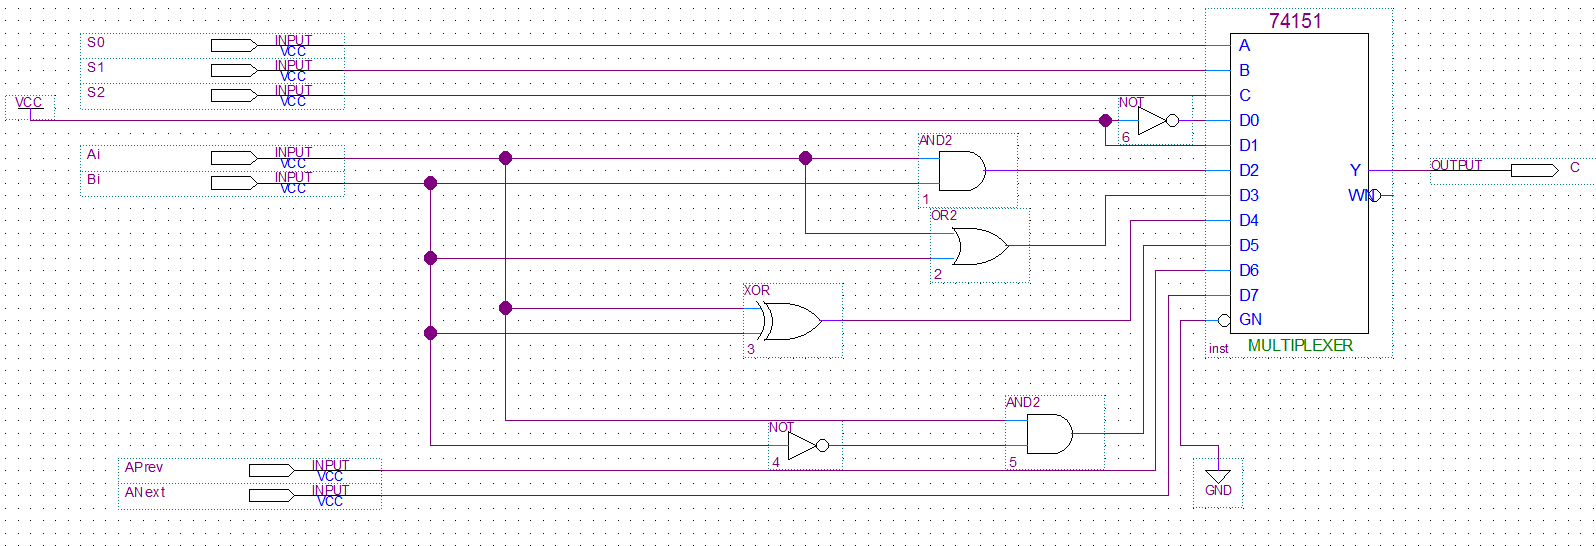
\includegraphics[width=\textwidth]{Diagrams/BlockDiagram_1bitISC.PNG} 
\caption{One-Bit Logic and Shift Circuit}
\label{fig:OneBitISC}
\end{figure}

\begin{figure}[H]
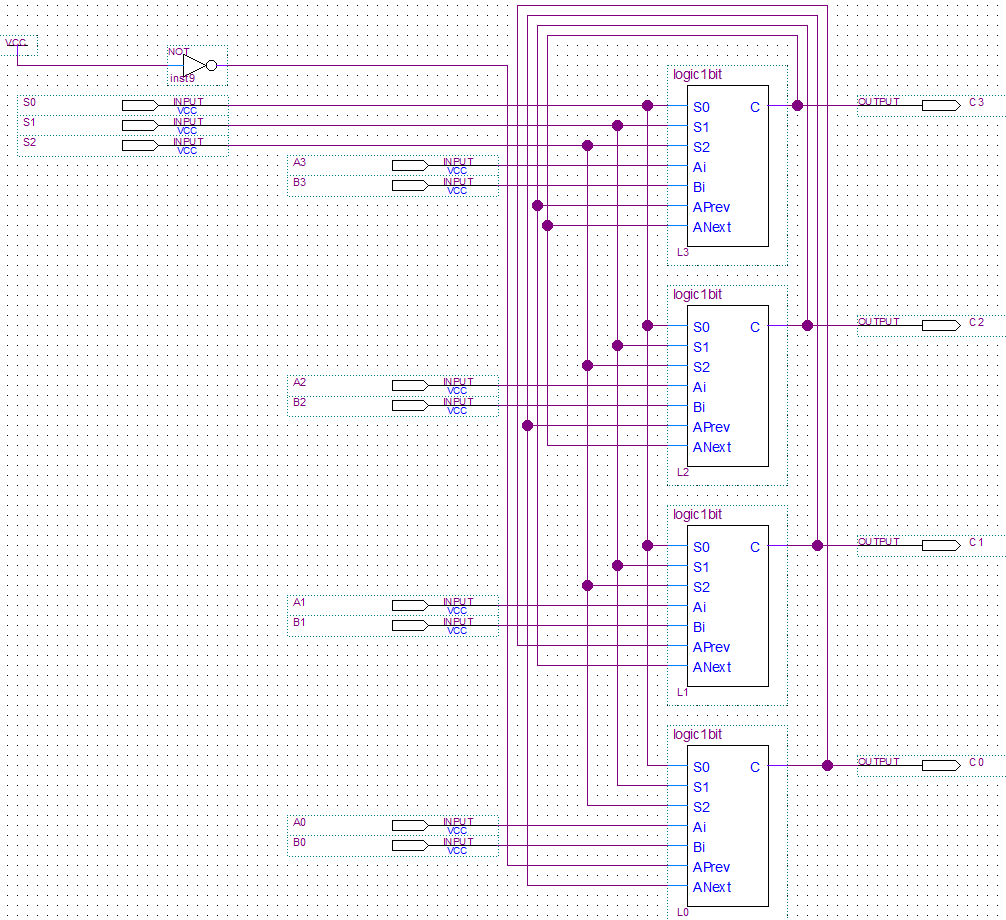
\includegraphics[width=\textwidth]{Diagrams/BlockDiagram_4bitISC.PNG} 
\caption{Four-Bit Logic and Shift Circuit}
\label{fig:FourBitISC}
\end{figure}

\begin{figure}[H]
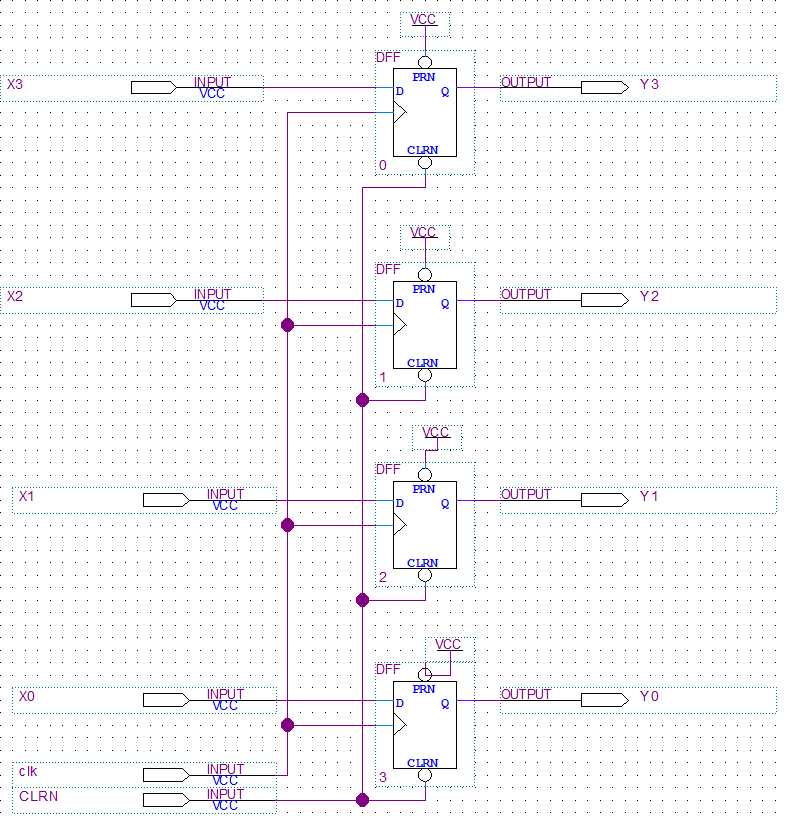
\includegraphics[width=\textwidth]{Diagrams/BlockDiagram_4BitRegister.PNG} 
\caption{Four-Bit Register}
\label{fig:FourBitRegister}
\end{figure}

\begin{figure}[H]
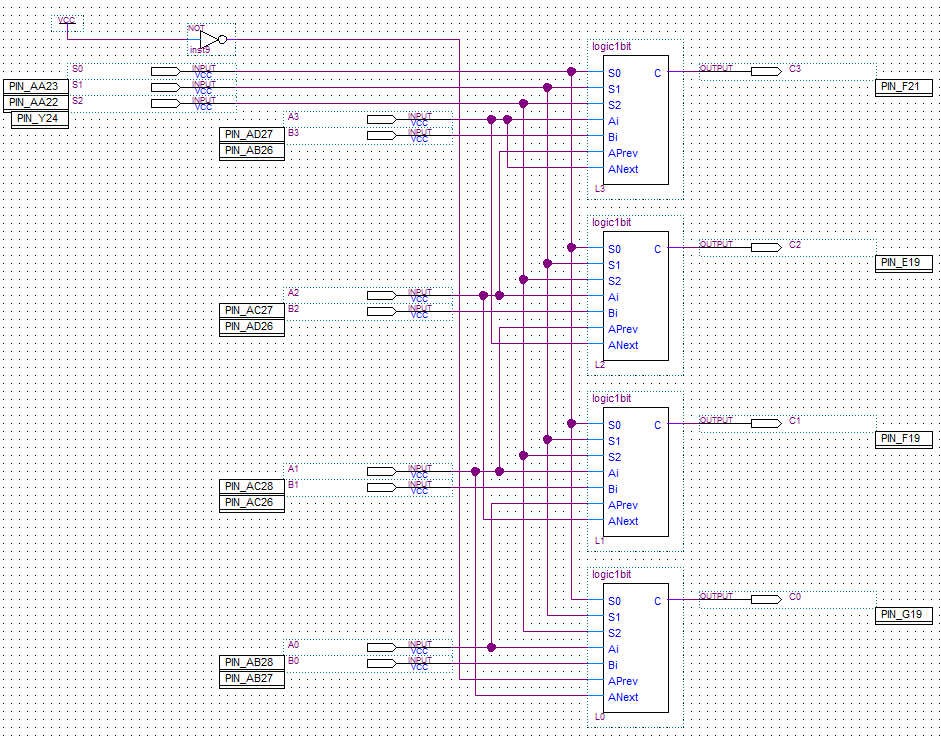
\includegraphics[width=\textwidth]{Diagrams/BlockDiagram_4BitRegister_VER2.PNG} 
\caption{Second Iteration of the Four-Bit Register}
\label{fig:FourBitRegisterSecondIteration}
\end{figure}

\begin{figure}[H]
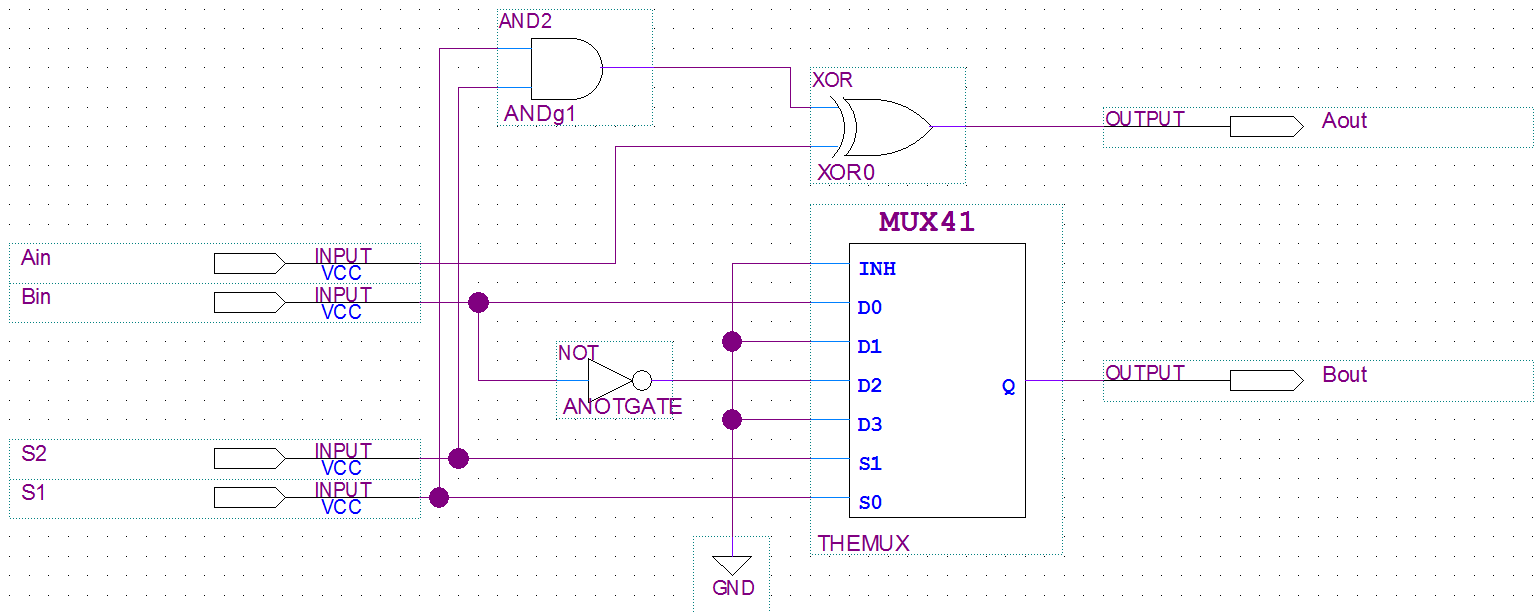
\includegraphics[width=\textwidth]{Diagrams/BlockDiagram_ABXIO.PNG} 
\caption{One-Bit Arithmetic Circuit "ABXIO"}
\label{fig:ABXIO}
\end{figure}

\begin{figure}[H]
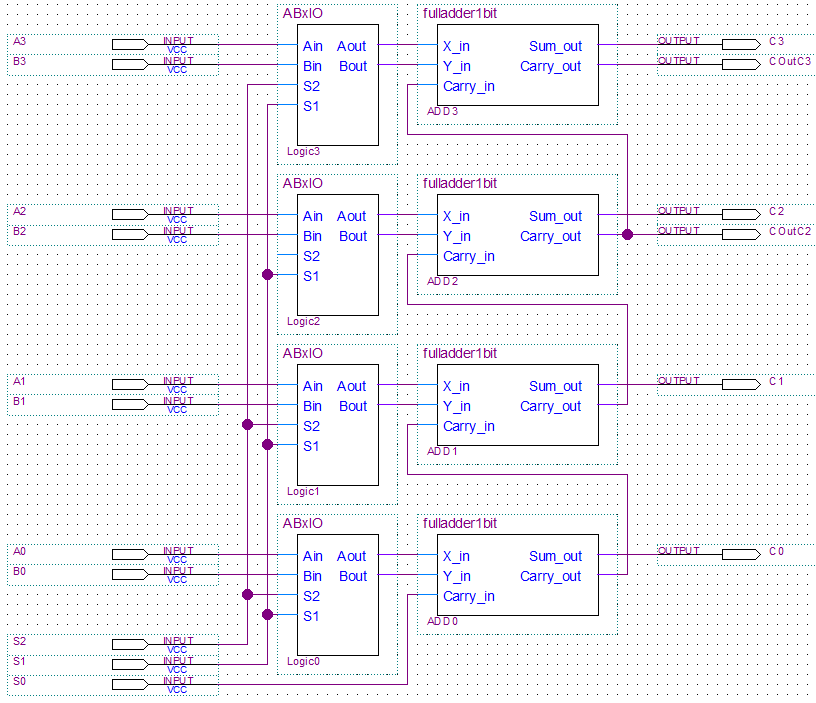
\includegraphics[width=\textwidth]{Diagrams/BlockDiagram_AC.PNG} 
\caption{Four-Bit Arithmetic Circuit}
\label{fig:AC}
\end{figure}

\begin{figure}[H]
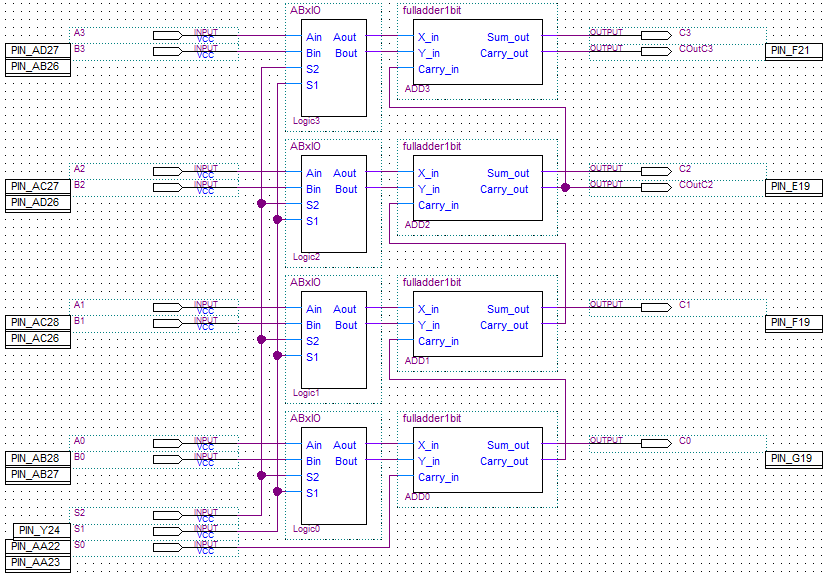
\includegraphics[width=\textwidth]{Diagrams/BlockDiagram_AC_VER2.PNG} 
\caption{Second Iteration of the Four-Bit Arithmetic Circuit}

\label{fig:ACSecondIteration}
\end{figure}

\begin{figure}[H]
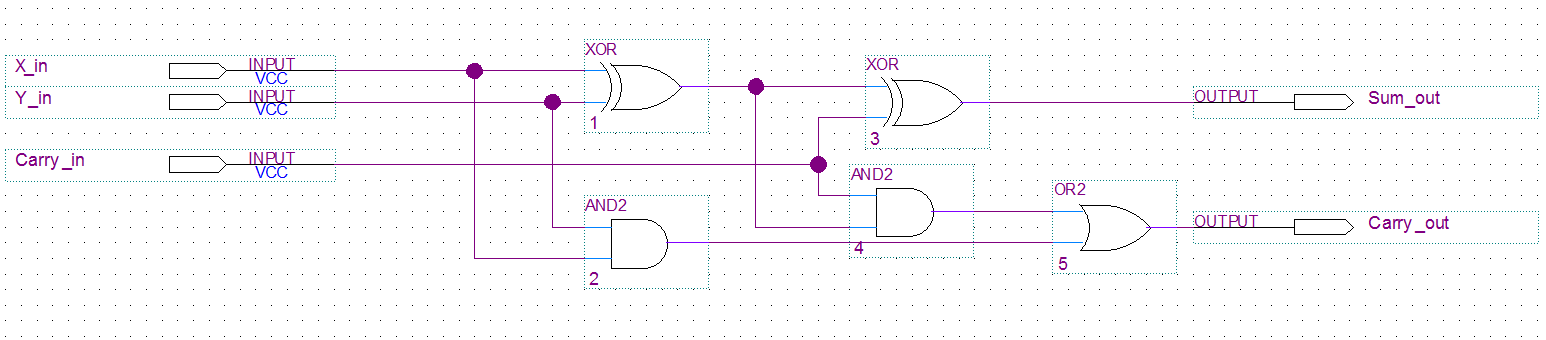
\includegraphics[width=\textwidth]{Diagrams/BlockDiagram_FullAdder.PNG} 
\caption{Full Adder}
\label{fig:FullAdder}
\end{figure}

\begin{figure}[H]
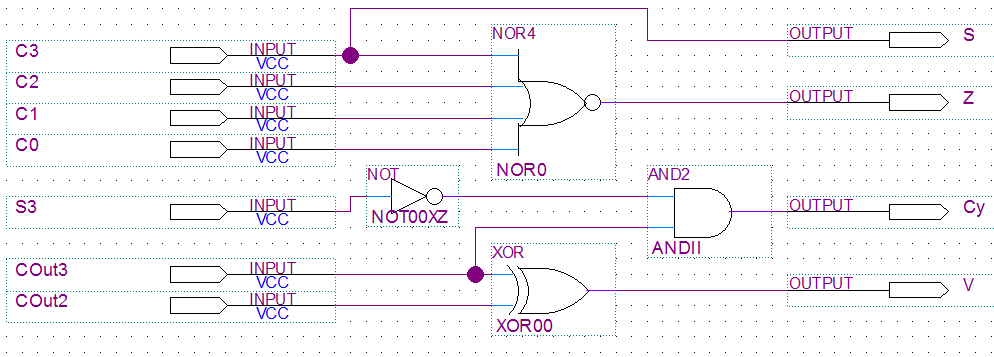
\includegraphics[width=\textwidth]{Diagrams/BlockDiagram_StateIV.PNG} 
\caption{Status Indicator Circuit}
\label{fig:StateIndicators}
\end{figure}

\subsection{Implemented Solution}

\begin{figure}[H]
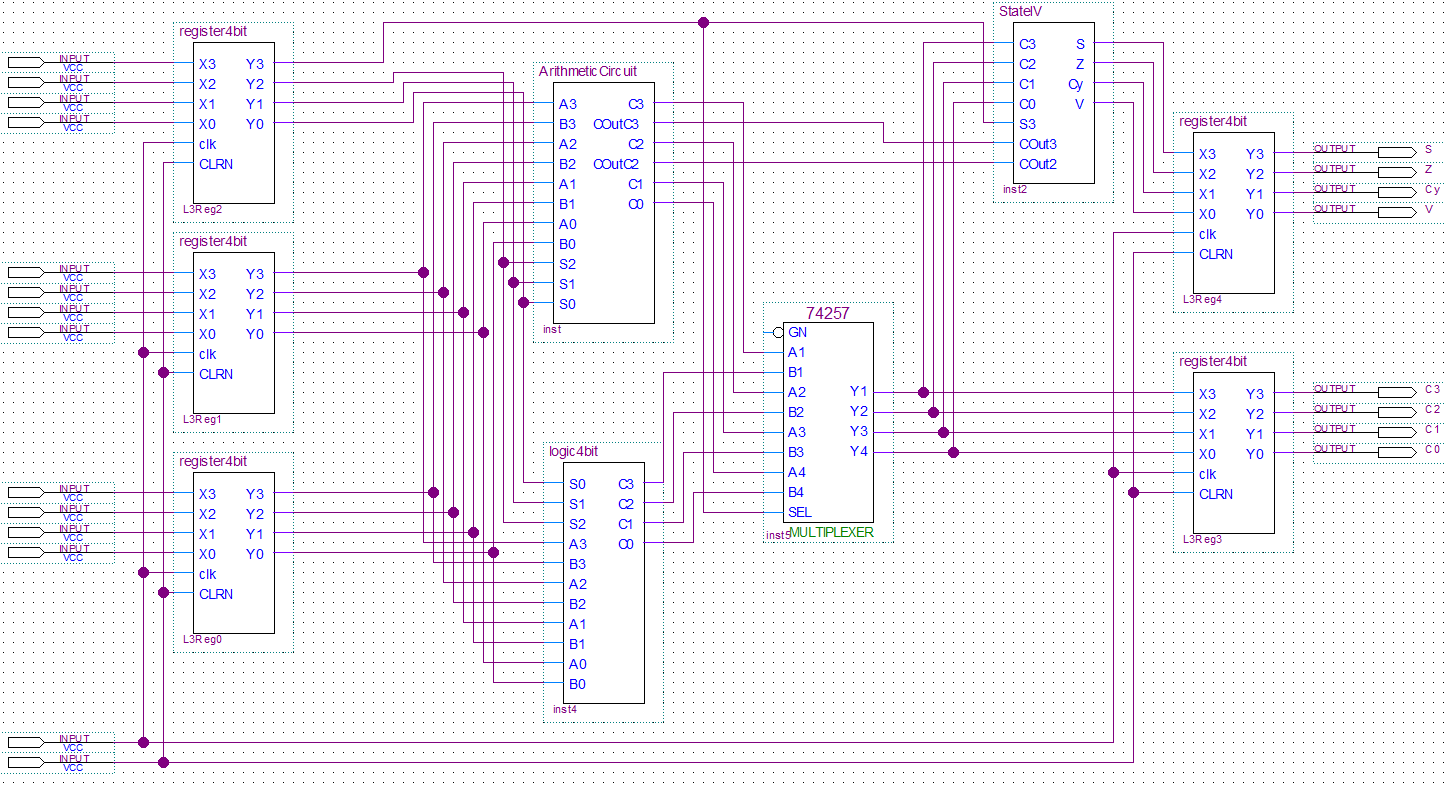
\includegraphics[width=\textwidth]{Diagrams/BlockDiagram_FULL_ALU.PNG} 
\caption{ALU}
\label{fig:ALU}
\end{figure}

\begin{figure}[H]
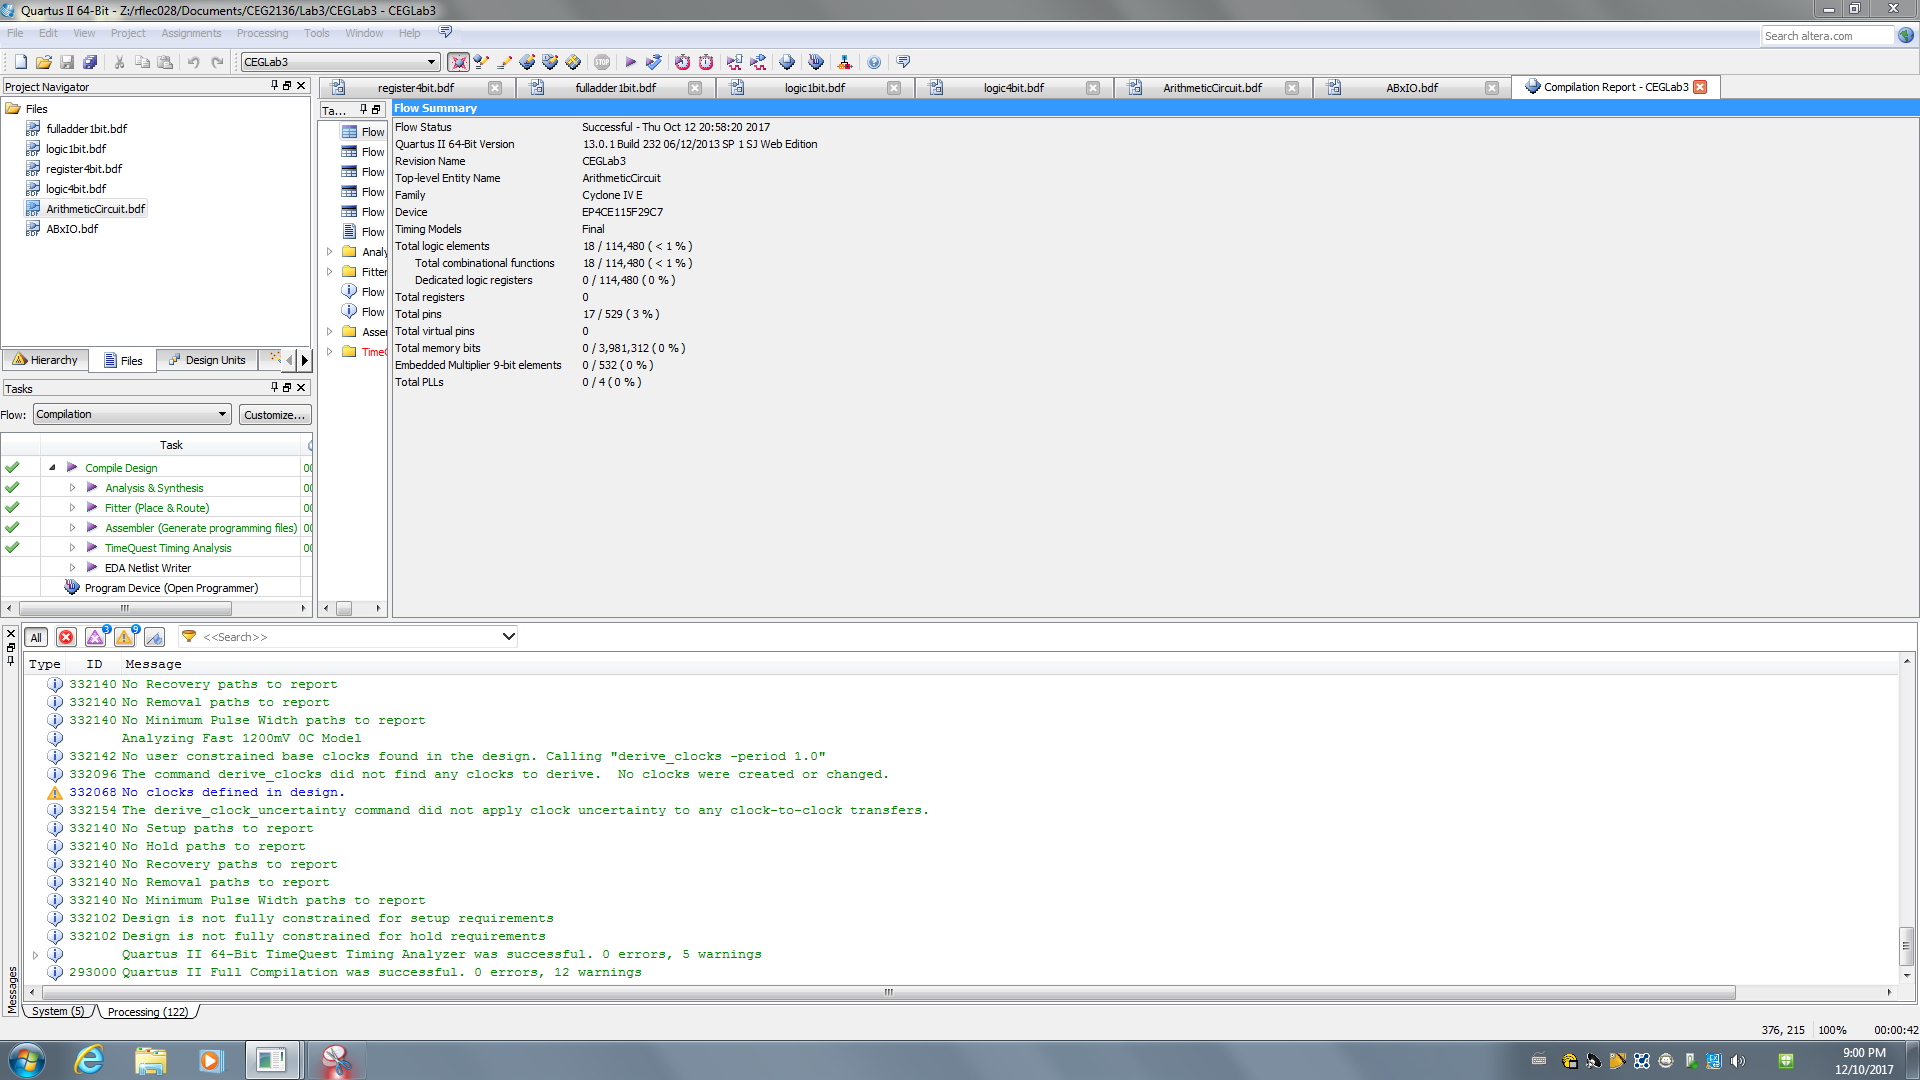
\includegraphics[width=\textwidth]{Diagrams/Diagnostics_CompilationReport.PNG} 
\caption{Successful Compilation}
\label{fig:compile}
\end{figure}

\newpage
\section{Implementation}

As seen in Figure \ref{fig:ALU}, our fully implemented ALU, we were able to successfully design and connect all of the lower-level circuits to create a functional final product.

\subsection{Simulation Results}

\begin{figure}[H]
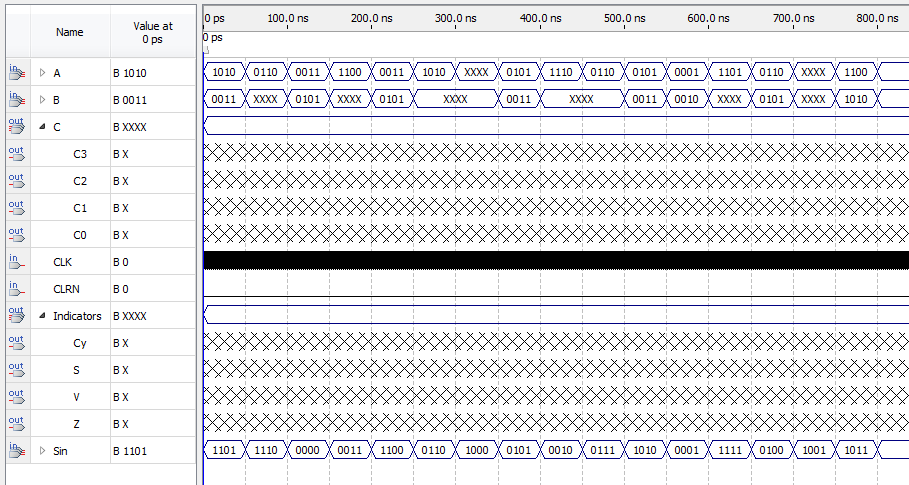
\includegraphics[width=\textwidth]{Diagrams/WaveFormSimFinalFailed.PNG} 
\caption{Complete Waveform File and Failed Waveform Generation}
\label{fig:wav2}
\end{figure}

As seen in the Figure \ref{fig:wav2} above, we were not able to run the waveform simulation on day 3 of the lab. The waveform generator worked well on the second lab day, but refused to run on the third, even when the project was transferred to 3 additional machines, a total of 4.

\begin{figure}[H]
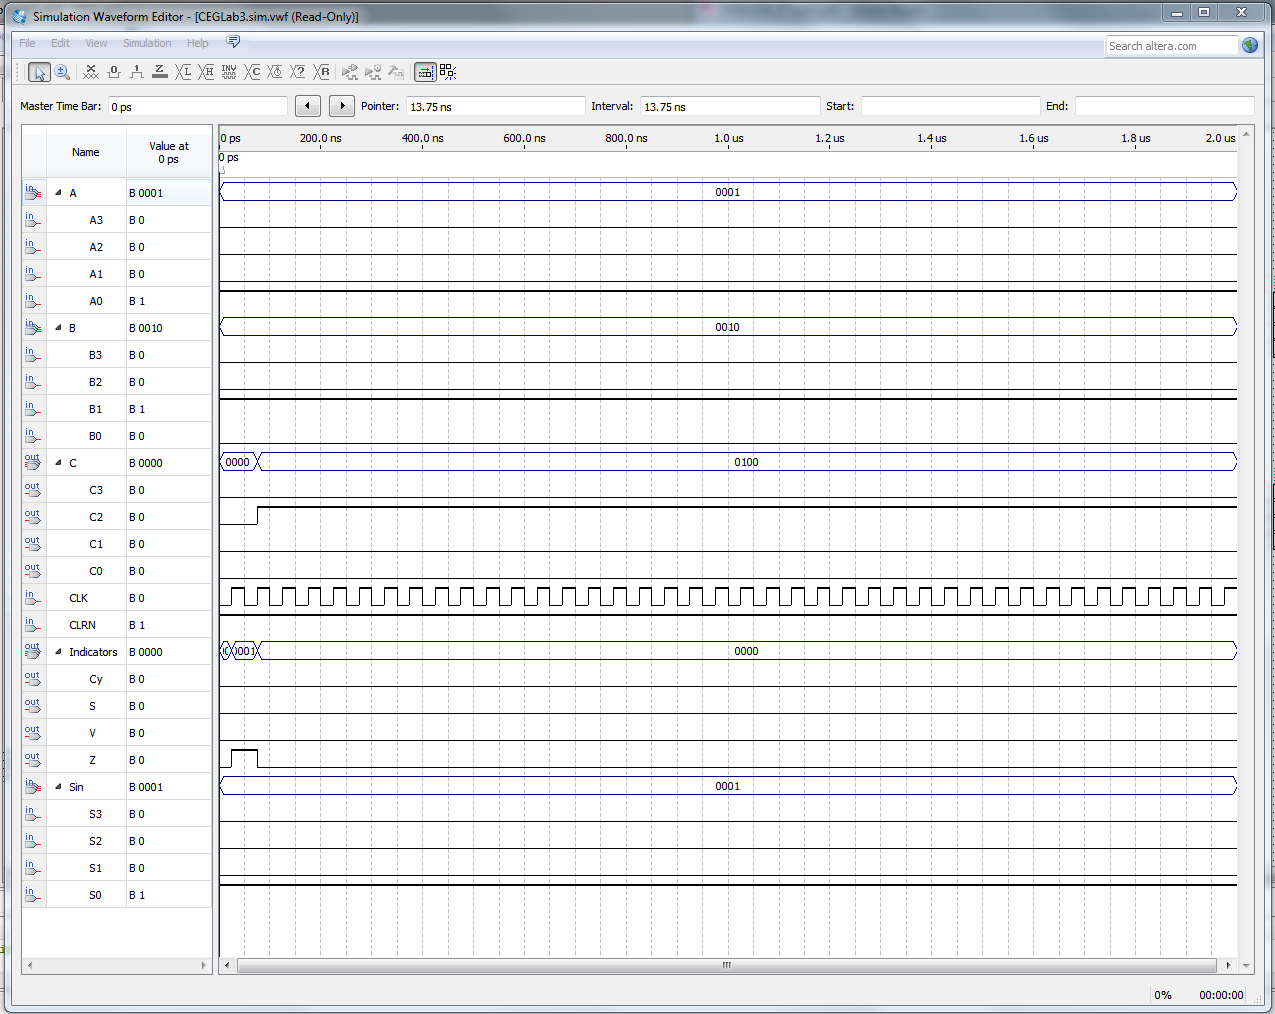
\includegraphics[width=\textwidth]{Diagrams/WaveFormSimulation.PNG} 
\caption{Single Successful Waveform Generation}
\label{fig:wav1}
\end{figure}

\newpage
\section{Design and Implementation Log}
\begin{enumerate}
\item When performing the pre-lab, our goal is not only to correctly implement the ALU circuits, but also to construct them in the most efficient way. Rather than implementing our one-bit AC module with an 8-to-1 multiplexer, we saw a very simple pattern for a, that pattern being (S2 and S1) XOR (Ain). This reduces the overall cost of the system. We have done all the circuit analysis before the lab, providing us plenty of lead during the first lab session, where we implemented all the block diagrams we need, naturally, it took considerable amount of time. We eventually managed to finish those diagrams and compiled them successfully. 
\item The second lab session was aimed to finish the testing and demo part of the lab, but when it came to the lab manual, there was a chart called Table 5: Sequence of micro-operations to simulate we had not even noticed. The chart was supposed be a part of pre-lab and be done in advance, the purpose of which is to compare the real outputs from the ALU we implemented and the answers on the chart to check possible flaws existed in the ALU. Without any choice, we had to take time filling out the chart and checking answers' correctness. After a period of time, we begin to assign pins and load the ALU circuit into the Altera board. When we played with the board, outputs of the LEDs assigned appeared to be acting strange, there was always a "0100" extra on every micro-operation that involved addition. That was when we knew there was a mistake. We went through the arithmetic part of the block diagrams from the 1-bit full adder and found out there was a connection missing in 4-bit arithmetic circuit. Later, when the logic operations were tested, we noticed that the shift function was not working as intended, and same again, we found our mistakes made in 4-bit register about the inputs of "APrev" and "ANext". Fixed and solved.
Two major mistakes were checked, and after going through Table 5 from start to end, our outputs from the Altera board were identical to the chart. 
\item The third lab session was about doing demo and performing waveform simulation for the Table 5. Unfortunately, we encountered an unknown bug which happened if we tried to import our existing lab3 project into \textit{Altera Quartus II} software, resulting in the failure of Table 5 waveform generation. After hitting run button, the waveform runtime window just popped out and closed instantly, not even entered the rendering process. This happened in several groups during the third lab session, we have tried switching work stations but the bug occurred again. Figure \ref{fig:wav1} is the only successful waveform result that we tested during the second lab session, where the waveform generator still worked.
\end{enumerate}
\newpage
\section{Discussion}

The only major point of discussion that has to be made relates to our testing, specifically the generation of simulated wave-forms.

In our testing on day 2, we ran every test case manually, on the  \textit{Altera DE2-115 FPGA}, in order to debug the circuit an iron out our issues. At the end of the lab, we began work on running the waveform, and simulated one set of inputs to ensure that the waveform was able to run. This test was successful, as shown in Figure \ref{fig:wav1}. Frustratingly, we were not able to replicate this test on the third day of the lab, where our only remaining task was to simulate the waveforms. Figure \ref{fig:wav2} shows our second waveform testing file, which we were never able to run. Conclusively, we apologize for the lack of a full waveform simulation in this lab report.

\subsection{Conclusions}

This lab was a general success. We were able to successfully design and implement a 1-bit full adder, 4-bit full adder, 1-bit LSC part, 4-bit LSC, a 4-bit register and our state monitoring circuit. These components were combined into a fully functional Arithmetic and Logic unit. When uploaded onto the Altera board, our design was able to reliably produce the correct output for the input given in the lab manual. While two major errors were encountered in testing, they were both quickly resolved by tracing the problem back to a component, and fixing the error. In one case, this was simply a missed connection. In another, the block was implemented incorrectly and a set of traces had to be deleted- but both mistakes were relatively minor. While only one test has a generated waveform, we did prove that the waveform output is correct as well, despite not having been able to test every function with a simulated waveform. Taking all of these things into account, it can be said that the lab was successful. The ALU was designed and tested successfully without many errors or setbacks, and the requirements of the lab were met.



\vspace*{\fill}
\center{\small Implemented by Ryan and Xiuzhu with \LaTeX and \TeX maker version 4.5.}

\end{document}





